\documentclass[a4paper,11pt]{article}
\usepackage[T1]{fontenc}
\usepackage[utf8]{inputenc}
\usepackage[italian]{babel}
\usepackage{amsmath,amssymb}
\usepackage{graphicx}
\usepackage{geometry}
\usepackage{xcolor}
\usepackage{listings}
\geometry{margin=2.5cm}

\lstdefinelanguage{MiniZinc}{
  morekeywords={int,set,of,array,var,constraint,include,solve,satisfy,output,show},
  sensitive=true,
  morecomment=[l]{\%},
  morestring=[b]"
}

\lstset{
  language=MiniZinc,
  basicstyle=\ttfamily\small,
  keywordstyle=\color{blue}\bfseries,
  commentstyle=\color{teal!70!black}\itshape,
  stringstyle=\color{orange!70!black},
  numbers=left,
  numberstyle=\tiny\color{gray},
  stepnumber=1,
  numbersep=8pt,
  showstringspaces=false,
  frame=single,
  breaklines=true
}

\title{CSP: Edge Colouring}
\date{}

\begin{document}
\maketitle

Dato in input un grafo non diretto $G = (V, E)$, si vogliono colorare gli archi del grafo
con 3 colori (denotati con $1$, $2$ e $3$) di modo che non esistano triangoli composti da
archi tutti dello stesso colore.

\subsection*{1.1 Modellazione} 
Una formulazione CSP ad alto livello è la seguente.

\paragraph{Variabili}
Definiamo una variabile per ogni arco:
\[
X = \{x_{uv} \mid (u,v) \in E\},
\]
dove $x_{uv}$ rappresenta il colore dell'arco che collega i vertici $u$ e $v$.
\paragraph{Domini}
\[
\forall x \in X:\quad D(x)=\{1,2,3\}.
\]

\paragraph{Vincoli}

Definiamo l'insieme dei triangoli di $G$ come 
\[
T = \{\{u,v,w\} \subseteq V \mid (u,v), (v,w), (w,u) \in E\}.
\]

Allora, per ogni triangolo $\{u,v,w\} \in T$, imponiamo il vincolo che i colori degli archi
$(u,v)$, $(v,w)$ e $(w,u)$ non siano tutti uguali:
\[
\forall \{u,v,w\} \in T:\quad \neg(x_{uv} = x_{vw} = x_{wu}).
\]

\newpage

\subsection*{1.2 Istanziazione per il grafo in figura}

\begin{figure}[h]
\centering
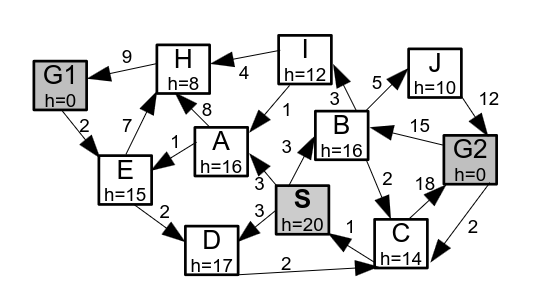
\includegraphics[width=0.6\textwidth]{graph.png}
\end{figure}


Si ottiene il CSP $(X,D,C)$:

\[
X = \{
x_{SA}, x_{SB}, x_{SC}, x_{SD}, x_{AE}, x_{AH}, x_{AI}, x_{BI}, x_{BJ}, x_{BC}, x_{BG2}, x_{CD}, x_{CG2}, x_{DE}, x_{EH}, x_{EG1}, x_{HG1}, x_{HI}, x_{JG2}
\}
\]

\[
\forall x \in X:\quad D(x)=\{1,2,3\}.
\]

\[
T = \{
  \{ S, B, C \},
  \{ S, C, D \},
  \{ A, E, H \},
  \{ A, I, H \},
  \{ G1, E, H \},
  \{ G2, B, J \},
  \{ C, B, G2 \}
  \}
\]

\[
\begin{aligned}
C = \{\,&\neg(x_{SB} = x_{BC} = x_{SC}),\\
      &\neg(x_{SC} = x_{CD} = x_{SD}),\\
      &\neg(x_{AE} = x_{EH} = x_{AH}),\\
      &\neg(x_{AH} = x_{HI} = x_{AI}),\\
      &\neg(x_{EG1} = x_{EH} = x_{HG1}),\\
      &\neg(x_{BG2} = x_{BJ} = x_{JG2}),\\
      &\neg(x_{BC} = x_{BG2} = x_{BJ})\,\}
\end{aligned}
\]

\newpage

\subsection*{1.3 Codifica in MiniZinc}
\begin{lstlisting}
int: n;                            % Numero di nodi
array[1..n, 1..n] of bool: adj;    % Matrice di adiacenza

% Variabili: color[i,j] e' il colore dell'arco (i,j), 0 se non esiste
array[1..n, 1..n] of var 0..3: color;

constraint forall(i, j in 1..n where i < j) (
    if adj[i,j] then color[i,j] > 0 else color[i,j] == 0 endif
);

% Simmetria: (i,j) == (j,i)
constraint forall(i, j in 1..n) (
    color[i,j] == color[j,i]
);

constraint forall(i, j, k in 1..n where i < j /\ j < k) (
    (adj[i,j] /\ adj[j,k] /\ adj[k,i]) -> 
        not (color[i,j] == color[j,k] /\ color[j,k] == color[i,k])
);

solve satisfy;
\end{lstlisting}

\end{document}